\documentclass[11pt]{scrartcl}
\usepackage[sexy]{evan}
\usepackage{graphicx}



\usepackage{answers}
\usepackage{listings}
\usepackage{xcolor}
\Newassociation{hint}{hintitem}{all-hints}
\renewcommand{\solutionextension}{out}
\renewenvironment{hintitem}[1]{\item[\bfseries #1.]}{}
\declaretheorem[style=thmbluebox,name={Theorem}]{thm}


\DeclarePairedDelimiter\ceil{\lceil}{\rceil}

\lstset{
    frame=tb, % draw a frame at the top and bottom of the code block
    tabsize=4, % tab space width
    showstringspaces=false, % don't mark spaces in strings
    numbers=left, % display line numbers on the left
    commentstyle=\color{green}, % comment color
    keywordstyle=\color{blue}, % keyword color
    stringstyle=\color{red} % string color
}

\begin{document}
\title{CS 170}
\author{Vishal Raman}
\thispagestyle{empty}
$ $
\vfill
\begin{center}

\centerline{\huge \textbf{CS 170 Lecture Notes, Fall 2020}}
\centerline{\Large \textbf{Algorithms and Intractable Problems} } 
\centerline{Professors: Avishay Tal, Umesh Vazirani}
\centerline{Scribe: Vishal Raman}
\end{center}
\vfill
$ $
\newpage
\thispagestyle{empty}
\tableofcontents
\newpage
%\maketitle
\section{September 1st, 2020}
\subsection{Naive Multiplication} 
Recall the example of Fibonacci: we went from a complexity of $O(2^n) \rightarrow O(n^2) \rightarrow O(f(n))$, where $f(n)$ is the runtime for multiplying $n$-bit numbers.  The naive algorithm is the usual multiplication algorithm for multiplying by hand.
\begin{center}
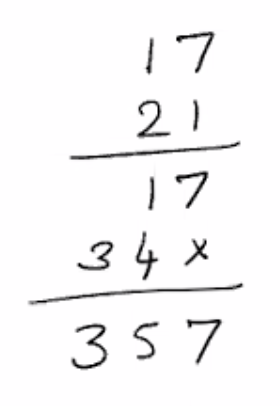
\includegraphics[scale=0.5]{multiply.png}
\end{center}
\begin{lstlisting}[language=python, caption={Naive n-bit multiplication}]
function multiply(x, y):
Input: n-bit integers, x, y, y >= 0
Output: Product

    if (y == 0) return 0;
    s = multiply(x, floor(y/2))
    if y is even:
    	return 2z
    else
    	return x+2z
\end{lstlisting}
If we write $x = \sum_{i=0}^{n-1} x_{j}2^i, y = \sum_{i=0}^{n-1} y_i 2^i$, so 
$$xy = \left (\sum_{i=0}^{n-1} x_{j}2^i\right )\left (\sum_{i=0}^{n-1} y_i 2^i\right ) = \sum_{j, k = 0}^n x_jy_k 2^{j+k}.$$
\subsection{Divide and Conquer: Karatsuba's Algorithm}
For a Divide and Conquer problem, we do the following:
\begin{enumerate}
\item  Break problem into pieces.
\item Solve pieces recursively.
\item Glue solutions of pieces to get solution of original problem.
\end{enumerate}
We first have $x$ an n-bit number that we break up into $x_L, x_R$, each $n/2$ bit numbers.  Similarly, we break $y$ into $y_L, y_R$.
\begin{center}
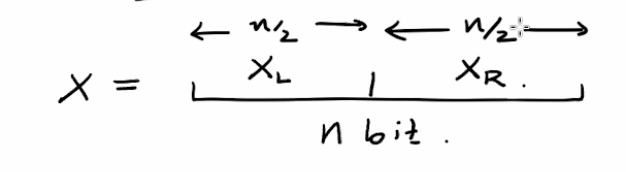
\includegraphics[scale=0.5]{dac.png}
\end{center}
Note that $x = 2^{n/2}x_L + x_R, y = 2^{n/2}y_L + y_R,$, so
$$xy = 2^n x_Lx_L + 2^{n/2}(x_Ly_R + x_Ry+L) + x_Ry_R.$$
We now have 4 multiplications, involving $n/2$-bit numbers.  Multiplication by $2^m$ can be shifting ($O(m)$ time), and addition is $O(1)$.  Hence, we have a recurrence equation for the runtime,
$$T(n) = 4T\left (\frac{n}{2}\right ) + O(n).$$
\begin{center}
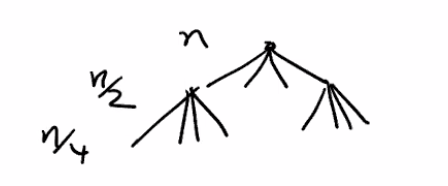
\includegraphics[scale=0.5]{rec.png}
\end{center}
Note that the depth of the recursion tree is $\log n$ and there are $4^{\log n} = n^2$ leaves.  But this would have the same runtime as the naive algorithm, so more work is required to optimize.

We note the following trick from Gauss:
$$(a+bi)(c+di) = (ac-bd) + (ad+bc),$$
and note that $$(a+b)(c+d) = (ac+bd) + (ad+bc),$$
so it suffices to compute $ac, bd, (a+b)(c+d)$, since $(a+b)(c+d)-ac-bd = ad+bc$, which is the other term.

We can apply the trick in the following way:
$$(2^{n/2}x_L + x_R)(2^{n/2}y_L + y_R) = 2^n x_Lx_L + 2^{n/2}(x_Ly_R + x_Ry+L) + x_Ry_R$$
and $$(x_L+x_R)(y_L+y_R) = x_Ly_L + x_Ry_R + (x_Ly_R+y_Lx_R).$$
Our new recurrence relation is
$$T(n) = 3T\left (\frac{n}{2}\right ) + O(n).$$
Now, the branching factor is only $3$, so the number of leaves is given by $$3^{\log n} = n^{\log 3}.$$

\subsection{Master Theorem}
We have the following method of solving recurrence relations:
\begin{thm}[Master Theorem] If $T(n) = aT(\ceil{n/b}) + O(n^d)$ for constants $a > 0, b > 1, d \ge 0$, then
$$T(n) = \begin{cases}
O(n^d) & \text{ if } d > \log_b a \\ 
O(n^d \log n) & \text{ if } d = log_b a \\
O(n^{\log_b a}) & \text{ if } d < log_b a
\end{cases}$$
\end{thm}
\pagebreak
\section{September 3rd, 2020}
\subsection{Sorting}
Recall merge sort: we have an array $a[1, \dots, n]$ and we want to sort the elements in non-decreasing order.  We run merge sort on each half, and merge the two halves by taking 2 pointers and picking the smallest element from one of the two halves.  Merge sort has a runtime of 
$$T(n) = 2T(n/2) + O(n) \Rightarrow T(n) = O(n \log n).$$

We now consider the problem of counting the number of inversions.  We define an \textbf{inversion} of an array $a$ to be a pair of indicies $i, j$ so that $i < j$ but $a[i] > a[j]$.  
\begin{center}
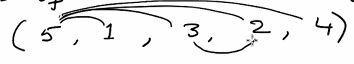
\includegraphics[scale=1]{inversion.png}
\end{center}
We will use a divide-and-conquer approach.  We split the two halves, and for each half, we count inversions and sort the halves.  

When calling the recursive operation on $a[1, \dots, n]$ it should return $b[1, \dots, n/2]$, the sorted left half and $k_1$, the number of inversions in the left half, $c[1, \dots, n/2]$ the sorted right half, and $k_2$ the number of inversions in the right half.  Then, when merging both halves, we can read off the number of inversions by counting the number of skipped elements in the right half when inserting elements from the left half.
\begin{center}
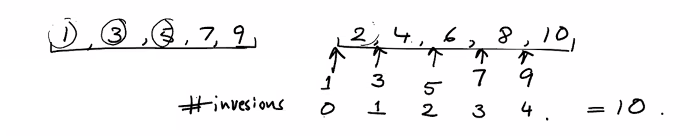
\includegraphics[scale=1]{countInv.png}
\end{center}
The merging operation takes $O(n)$, and we would like $T(n) = 2T(n/2) + O(n)$ to get a runtime of $T(n) = O(n \log n)$.  Proof of correctness can be done by induction on $n$, which is left as an exercise.  

Can we do better than $O(n \log n)$?  As an abstraction, consider an array $a[1, \dots, n]$. 
 We can make a query $a(i) > a(j)$ for each $i, j \in\{1, \dots, n\}$, for $i < j$.
\begin{center}
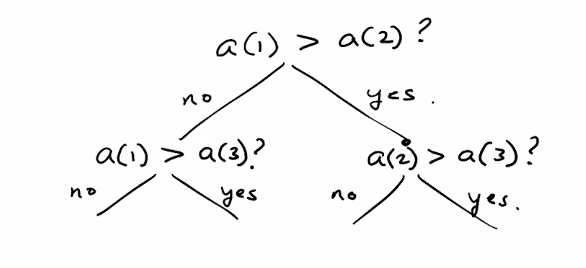
\includegraphics[scale=1]{sort.png}
\end{center}
In order to have a proper sorting algorithm, each leaf must contain exactly one permutation.  Hence, the number of leaves is at least $n!$, the number of permutations with $n$ elements.  The height of the tree(which is the worst case runtime), is given by $$\Omega(\log n!) = \Omega(\log (n/e)^n) = \Omega(n \log n).$$
\subsection{Median Finding}
Suppose we have an array $a[1, \dots, n]$.  We wish to find the median of the list.  

Suppose we can pick out some element $\ell$ between $n/4$ and $3n/4$ in the sorted list.  If we make $n$ comparisons with the element, we'd know how many elements are less than the element and how many are larger than it, so we'd know which half contained the median (either $[1, \ell]$ or $[\ell+1, n]$).  
\begin{center}
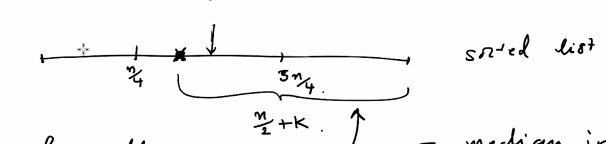
\includegraphics[scale=1]{median.png}
\end{center}
If $k < n$, then find the k-th smallest element in the left half.  Otherwise, find the $k-n$-th element in the right half.  We have the following recurrence,
$$T(n) \le T(\frac{3n}{4}) + O(n) \Rightarrow T(n) = O(n).$$

To actually do this, pick some element at random.  We can show the expected number of times it takes to pick a proper element is $2$.  So, redefine $T(n)$ is be the expected time to find the $k$-th smallest in $n$ element array.

Suppose the time to find the element is $T_1 = n$. Then, the time to find the next element is $T_2 = (3/4)n$, the next would be $T_3 = (3/4)^2n$, so we obtain a geometric series $T = \sum T_i = O(n)$.

Now, $E[T_1] = 2n, E[T_2] = 2(3/4)n, \dots$.  Note that 
$$E(T) = E(\sum_{i=1}^d T_i) = \sum E(T_i) = O(n),$$
by linearity of expectation.

Suppose $P[+1] = p$ and $W$ is the waiting time for a heads.  $$E(W) = p + (1-p)(1+E(W)) = 1 + (1-p)E(W) \Rightarrow E(w) = \frac{1}{p}.$$

\subsection{Matrix Multiplication}
We are given two $n$ by $n$ matrices $X, Y$, and we would like to compute $XY = Z$.   This is naively $O(n^3)$:
\begin{center}
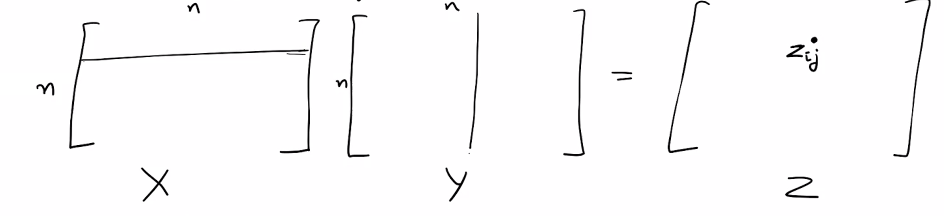
\includegraphics[scale=.75]{matrix.png}
\end{center}
Note that
$$Z_{ij} = \sum_{k=1}^n X_{ik}Y_{kj}.$$

We try a divide-and-conquer approach.  Split $X$ and $Y$ as follows:
\begin{center}
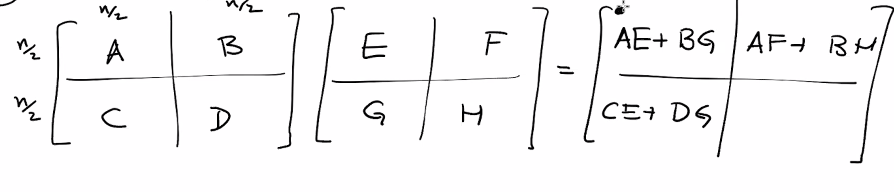
\includegraphics[scale=.75]{split.png}
\end{center}
Then,
$$T(n) = 8T(n/2) + O(n^2) \Rightarrow T(n) = O(n^3).$$

This has lower constant factors due to memory accessing, but the runtime can be further improved with Strassen's algorithm:
\begin{center}
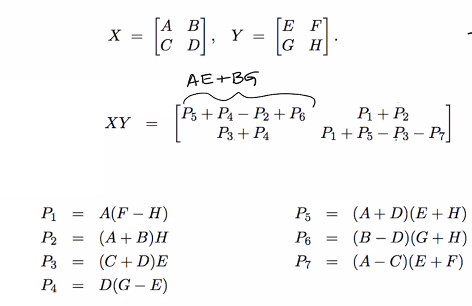
\includegraphics[scale=1]{strassen.png}
\end{center}
\end{document}
